\documentclass[letterpaper]{article}
\usepackage{aaai}
\usepackage{times}
\usepackage{helvet}
\usepackage{courier}
\usepackage{amsmath,amssymb,amsthm,fullpage,mathtools}
\usepackage{mathtools}
\usepackage[english]{babel}
\usepackage{graphicx}
\usepackage{fontspec}
\usepackage{newunicodechar}
\usepackage{multicol}
\usepackage[margin={1.5cm,1.5cm}]{geometry}
\usepackage{hyperref}
\DeclareMathOperator*{\argmax}{\arg\!\max}
\setlength{\pdfpagewidth}{8.5in}
\setlength{\pdfpageheight}{11in}

\usepackage{tikz} % for dependency graph
\usepackage{listings} % to include code

% for bibliographic information
\usepackage{biblatex}
\bibliography{report.bib}


% /Author (Kevin K. Eskici, Luis A. Perez, Aidi Zhang)}
\setcounter{secnumdepth}{0}

% we want to adjust the seperationg between columns
\setlength{\columnsep}{1cm}

% set all paragraphs to no indent
\setlength\parindent{0pt}

\title{Practical 4: Reinforcement Learning with Swingy Monkey}
\author{Kevin Eskici\thanks{keskici@college.harvard.edu}, Luis A. Perez\thanks{luisperez@college.harvard.edu}, Aidi Zhang\thanks{aidizhang@college.harvard.edu} \\
Computer Science 181, Harvard University}

\date{\today} 

\begin{document}

\maketitle

\begin{abstract}
\begin{quote}
This paper explores model-free, model-based, and mixture models for reinforcement learning under the setting of a SwingyMonkey game \footnote{The code is hosted on a public repository \href{https://github.com/kandluis/machine-learning}{here} under the prac4 directory.}. SwingyMonkey is a simple game with well-defined goals and mechanisms, with a relatively small state-space. Using Bayesian Optimization \footnote{The optimization took place using the open-source software made available by HIPS \href{https://github.com/HIPS/Spearmint}{here}.} on a simple Q-Learning algorithm, we were able to obtain high scores within just a few training epochs. However, the system failed to scale well after continued training, and optimization over hundreds of iterations proved too time-consuming to be effective. After manually exploring multiple approaches, the best results were achieved using a mixture of $\epsilon$-greedy Q-Learning with a stable learning rate,$\alpha$, and $\delta \approx 1$ discount factor. Despite the theoretical limitations of this approach, the settings, resulted in maximum scores of over 5000 points with an average score of $\bar{x} \approx 684$ (averaged over the final 100 testing epochs, median of $\bar{m} = 357.5$). The results show an continuing linear log-relation capping only after 20,000 training epochs.    
\end{quote}
\end{abstract}

\section{Introduction}
\label{sec:introduction}
Recent advancements in reinforcement learning have led to an increase in activity in the field. In particular, three main approaches have surfaced \cite{rl_lecture}. 

\subsection{Overview of Reinforcement Learning}
The first approach can be thought of model-based reinforcement learning in which the agent, in our particular case termed Monkey, attempts to learn a model of the world. Learning a model is as simple as learning the transition probabilities for each $(s,a,s')$ triplet in the world, where $s,s' \in \mathcal{S}$ are predefined states (labeled $P$). We also have that action $a$ at state $s$ leads to $s'$ with some non-zero probability. The essence of the model based-approaches is to learn these probabilities. In addition, the model based approach also learns a model of the rewards received at each state-action tuple, $R$. Once the model $(P,R)$ is known, training occurs in the form of finding the optimal policy, $\pi^*$, which is typically accomplished using either Policy Iteration or Value Iteration as described by Avi Pfeffer \cite{mdp_lecture}. Typically, the agent is allowed a phase or episode of a certain number of epochs during which he uses the previous optimal policy $\pi_i^*$ to make decisions. At the end of each episode, the agent now has a better model of the world and performs an optimization on this new model, leading to 
\[
\pi_{i+1}^* \leftarrow \text{OPT}\{(P,R)_i\}
\]
where $(P,R)_i$ is the currently learned model.\\

A second approach is the well-known and often-used Q-Learning Algorithm. This is a model-free learning mechanism which only implicitly learns transition probabilities through the maximization of the $Q: \mathcal{S} \times \mathcal{A} \to \mathbb{R}$ function. The objective is to take the rewards obtained from different sequences of actions in particular states as samples in approximating the true total value of a state-action tuple $(s,a)$, given by $Q(s,a)$. The approach is theoretical grounded in the idea of stochastic gradient ascent, and typically involves a learning rate parameter $\alpha > 0$ which can be tweaked, as we do in this paper, to improve the rate of convergence onto an optimal policy (convergence is not always guaranteed). The simplicity with which Q-Learning can be implemented is surprising, as it is the method which led to some of the best results after optimizing the parameters.\\

A third approach utilizes a mixture of model-free and model-based learning. While the model-based approach learns a model of the world and then solves for an optimal action policy $\pi^*$, a method known as Temporal Difference Learning does away with finding the optimal policy. It instead collects information on the world, developing a model $P$ of transition probabilities on state-action-state triplets and a model $R$ of the rewards for each state-action tuple. It then uses an approach where it attempts to estimate the value function $V(s)$ for each $s \in \mathcal{S}$. This leads to faster propagation of negative rewards, and typically faster learning. Once the value function has been defined, the action of choosing the optimal policy involves a simple expectation maximization procedure.
\\
Lastly, in this paper we also introduce the topic of parameter optimization through Bayesian optimization, as discussed by Snok, Larochelle, and Adams \cite{bayes}. TD Learning and Q Learning were both heavily optimized, and model based learning only slightly so. While the theoretical properties of convergence of both model-based and TD learning would have led us to belief in them performing better , we actually found that Q-Learning, along with Bayesian Optimization of the parameters, led to both an incredibly short training epoch (under 10 epochs) as well as an impressively robust, long-term model.

\subsection{SwingyMonkey}
SwingyMokey is a simple game, similar in kind to the popular, now defunct, FlappyBird \footnote{Information on FlappyBird and online version of the game can be found \href{http://flappybird.io/}{here}.}. The mechanics of the game are simple, and are discussed in more detail in Section \ref{sec:methods}. The purpose of the game is to cross have the Monkey cross through as many tree ``gaps'' as possible by ``swinging'' from branch to branch.

In this paper, we explore described reinforcement learning approaches and provide both a theoretical foundations as well as experiment results. The code for the simulations is open-source and available on gitHub (git@github.com:kandluis/machine-learning.git). Where deemed relevant, we present snippets from the code.

\section{Methods}
\label{sec:methods}
In this section, we introduce a thorough representation of the game dynamics as well as in-depth theoretical foundations for the RL methods utilized. Additionally, we discuss the parameters for each method and their expected effect on training. We finalize the section with a short discussion on parameter optimization through the use of the Spearmint software package.

\subsection{SwingyMonkey Mechanics}
We now introduce the mechanics of the SwingyMonkey game, as well as a description of parameters used throughout the models described in subsequent sections. 

\begin{figure}
\centering
\includegraphics[scale=0.3]{swingymonkey}
\caption{The SwingyMonkey game windows, with different state parameters labeled.}
\label{fig:swingymonkey}
\end{figure}

In Figure \ref{fig:swingymonkey}, we have the SwingyMokey game window. Looking at the image, we see that we actually have access to a total of seven variables for use in the description of the state space. The window size used for the monkey were $600 \times 400$\footnote{Other parameters utilized are defined in \textbf{parameters.py}.}.

Reward definitions are as follows:
\begin{itemize}
\item Reward of +1 for passing a tree trunk
\item Reward of -5 for hitting a tree trunk
\item Reward of -10 falling out of the game screen
\end{itemize}
At this point, it's of interest to note that the above rewards are well geared for negative reward propagation in Q-Learning. Q-Learning tends to suffer from the inability to propagate negative rewards quickly (due to the maximization aspect of the propagation, which tends to favor positive values). \\

The first challenged in the training of the monkey the bucketing of the above state space in order to facilitate learning. While it is possible to train on a large state space, faster learning can occur with a smaller set of feasible states. Additionally, some states are redundant. It's not necessary to know the absolute location of the monkey or the trees. Given that the tree itself never moves off screen in the vertical direction, simply having the distance from the monkey to the tree vertically and horizontally should be enough. We therefore define our states $s \in \mathcal{S}$ as $s = (h,w,v)$ (triplets) of three values. Let $d_v$ be the vertical distance in pixels of the the monkey from the tree, $d_h$ be the horizontal distance, and $v_m$ be the reported vertical velocity of the monkey in pixels per second. The values are given by:
\begin{align}
h &= \text{round}(d_h/p_h) \\
w &= \text{round}(d_w/p_w) \\
v &= \text{round}(v_m/p_v)
\end{align}
where $p = (p_h,p_w,p_v)$ is our current parameter vector. Intuitively, the value $p_w \times p_h$ defines a discretization of the screen into buckets of that dimension. The parameter $p_v$ does the same thing for the possible values of the velocity. With this definition, not only have we reduced the state space, we have introduced just three parameters which allow use to tweak the total size of the state-space. Naively, we would expect smaller state-spaces to learn more quickly but perform more poorly than larger state spaces. \\

Given the above definition of our parameterized state space, from now on referred to as $\mathcal{S}$ for succinctness, we now focus on defining the action space, $\mathcal{A}$. In the case of SwingyMokey, the action space is relatively simple, with only two possible actions in every state, ``jump'' and ``no jump''. For simplicity, we will define this action space as $\mathcal{A} = \{0,1\}$ where $0$ corresponds to ``no jump'' and $1$ to ``jump''.\\

The goal of the monkey is to receive as high a reward as possible, which is directly correlated with how many trees is can successfully pass without dying. The monkey is always attempting to maximize his reward, with the exception of a few of our implementation which include an $\epsilon$-greedy approach.\\

For the above reasons, we chose to consider this problem in the general case. We define then our reward function in terms of the total reward that the monkey obtains after $T$ ticks of the clock (which is how often Monkey reports his state and reward).
\begin{align}
R_{total} &= \lim_{T \to \infty} \sum_{t=1}^T R(s_t,a_t)
\end{align}
With the above in mind, we have generalized our problem to a infinite horizon reinforcement learning problem.


\subsection{Models}
\subsubsection{Model-based Learning}
\label{sec:model-based_learning}

As discussed in by Pfeffer \cite{mdp_lecture}, RL can be thought of as a Markov decision process. We can therefore attempt to learn by first creating a model for the world. We label our approximation for the model at episode $i$ as $\mathcal{M}_i = (P_i,R_i)$ where $P_i: \mathcal{S} \times \mathcal{A} \times \mathcal{S} \to [0,1]$ and $R_i: \mathcal{S} \times \mathcal{A} \to \mathbb{R}$ are our summaries of our collected statistics (the transition probabilities and the rewards). This information can easily be collected, and we do so, during the each action of the monkey takes \footnote{See \textbf{tdlearner.py} (from whom \textbf{modelbased.py} inherits).}. We keep a running total of:
\begin{align}
R_{\text{total}}: \mathcal{S} \times \mathcal{A} \to \mathbb{R} \label{eq:total_reward}\\
SA_{\text{total}}: \mathcal{S} \times \mathbb{A} \to \mathbb{N}\label{eq:sa_count} \\
SAS_{\text{total}}: \mathcal{S} \times \mathcal{A} \times \mathcal{S} \to \mathbb{N} \label{eq:sas_count}
\end{align}
The purpose of Function \ref{eq:total_reward} is to simply keep a running total of the rewards received for each state-action tuple. Similarly, Function \ref{eq:sa_count} keeps a running count of the number of times state $s \in \mathcal{S}$ has been visited and action $a \in \mathcal{A}$ has taken place. Lastly, Function \ref{eq:sas_count} keeps count of the number of times that state $s' \in \mathcal{S}$ has been reached after taking action $a$ from state $s$. \\

With these parameters, it becomes possible to reconstruct the model \footnote{See \textbf{tdlearner.py} for more information.}. The parameters can be estimated using the formulas:
\begin{align}
\mathbb{E}[R(s,a)] &= \frac{R_{\text{total}}(s,a)}{SA_{\text{total}}(s,a)}\\
P(s,a,s') &= \frac{SAS_{\text{total}}(s,a,s')}{SA_{\text{total}}(s,a)} 
\end{align}
We now have a way to approximate our transition model, $\mathcal{M}$. Therefore, after each epoch, our implementation of model-based learning \footnote{The implementation of the model based learning class can be found in \textbf{modelbased.py}.} simply needs to calculate the optimal policy, $\pi_i^*: \mathcal{S} \to \mathcal{A}$. This can be done using either Value Iteration or Policy Iteration. For factors of simplicity, our implementation make use of Value Iteration to approximate the best policy. Our initial policy is defined as $\forall s \in \mathcal{S}$:
\begin{align}
\pi^*_0(s) = 0
\end{align}

In addition to the paramers defined previously, model based learning also takes as input a discount rate, $\gamma$. \\

Model based learning is theoretically able to learn faster. However, it runs into issues of over-exploitation rather than exploration. Our simple implementation does not address these issues directly, though it's possible to do so using something like $\epsilon$-greedy learning or Boltzmann temperature learning. \\

The results of our implementation can be found in the file \textbf{modelbased.py}. The model can be used using the command:
\begin{verbatim}
@:	python run.py --live-train=50 ModelBased 
\end{verbatim}

\subsubsection{TD-Learning}
\label{sec:td-learning}
In addition to a model-based learner, we also implemented a mixed approach termed Temporal Difference Learning \footnote{A good explanation of TD-Learning can be found at \href{http://en.wikipedia.org/wiki/Temporal_difference_learning}{Wikipedia}.}. The theory behind temporal difference learning is that rather than calculating an optimal policy every episode, as is done in model-based learning, requiring the use of either Policy Iteration or Value Iteration, it is possible to instead sample the rewards and perform stochastic gradient ascent on the value function, $V: \mathcal{S} \to \mathbb{R}$. For each $s \in \mathcal{S}$, we have that $V(s)$ is the expected value of the state. If we can approximate the value function, then at each step, we can choose the optimal policy:
\begin{align}
\pi^*(s) &= \argmax_{a \in \mathcal{A}} \left[R(s,a) + \gamma \sum_{s' \in \mathcal{S}} P(s,a,s')V(s')\right] \label{eq:value_opt}
\end{align}
Intuitively, Equation \ref{eq:value_opt} simply attempts to pick the action $a$ which maximizes our expected reward. The reward we receive now, plus the expected reward from whatever new state $s'$ we transition into. The action is then the optimal. How does one approximate the function $V$. Note that by the above, we can actually consider $V(s)$ to be a random variable, and borrowing ideas introduced in the Q-Learning Section, we can generate the following update rule for the value on visiting state $s'$ and receiving reward $r$:
\begin{align}
V(s) &= V(s) + \alpha\left[(r + \gamma V(s')) - V(s) \right]
\end{align}
where we can note that $r + \gamma V(s')$ is the sample for $V(s)$, and $\alpha$ is a new parameter, the learning parameter, which we use to control the importance of new observations. \\

The advantages of TD-Learning over Model-Based learning lies in the simplicity of implementation of TD-Learning (you don't need to implement either Policy Iteration or Value Iteration). The disadvantage, of course, is that the model might not learn quickly enough. Due to the $\alpha$ factor, there exists some level of exploration that occurs. However, the risk of exploitation is still present, so introducing an $\epsilon$-greedy approach is still recommended with this approach.\\

The results of our implementation can be found in two files, \textbf{tdlearner.py} and \textbf{tdlearnerbayes.py}. The models can be run one after the other using:
\begin{verbatim}
@: python run.py [opts] TDLearner TDLearnerBayes
\end{verbatim}

\subsubsection{Q-Learning}
\label{sec:q-learning}
Q-Learning is a model free approach to reinforcement learning. In fact, this is the approach we found the most successful for our problem, and is therefore the one for which we made the most optimization and attempted the most number of iterations. We begin our discussion with the theory behind Q-Learning. Reinforcement learning can be thought of as simply attempting to solve for the function $Q: \mathcal{S} \times \mathcal{A} \to \mathbb{R}$. Once this function has been obtained, the task of calculating the optimal actions is simple:
\begin{align}
\pi^*(s) &= \argmax_{a \in \mathcal{A}} Q(s,a)
\end{align}

Q-learning takes the approach of stochastic gradient ascent, which makes sense in the problem setting given that the rewards received can be taken to be samples from a distribution. Recalling the definition of the Q function for the infinite horizon case with $\gamma$ as the discount factor, we have:
\begin{align}
Q(s,a) &= R(s,a) + \gamma\sum_{s'}P(s' \mid s,a)\max_{a'\in\mathcal{A}} Q(s',a') \\
&= R(s,a) + \gamma \mathbb{E}_{s'}\left[\max_{a\in \mathcal{A}}Q(s',a') \right] \\
&= \mathbb{E}_{s'} \left[R(s,a) + \gamma\max_{a \in \mathcal{A}} Q(s',a') \right]
\end{align}
where we have defined $P(s' \mid s,a)$ as the probability of transitioning into state $s' \in \mathcal{S}$ given that we take action $a \in \mathcal{A}$ from state $s \in \mathcal{S}$. If we take the above look at $Q$, an approximation can be done relatively simply. On each transition to a new state $s' \in \mathcal{S}$, we can simply update our value for $Q(s,a)$ for our previous state $s$ and our previous action $a$ given our new observation of the reward, $r + \gamma \max_{a' \in \mathcal{A}}Q(s',a')$:
\begin{align}
Q(s,a) \leftarrow Q(s,a) + \alpha\left[(r + \max_{a' \in \mathcal{A}}Q(s',a')) - Q(s,a) \right] \label{eq:q_update}
\end{align}
The intuition for this is that we're updating our current estimate of $Q(s,a)$ by our observed sample of the value of $Q(s,a)$. We have now extended our set of possible parameters further with the following:
\begin{align}
p &= p \circ [\gamma, \alpha]
\end{align}
This simple implementation of Q-Learning can be found in the file \textbf{qlearner.py}. 

Something of particular interest, however, is the learning rate $\alpha$ used by our model. In particular, the code in \textbf{qlearner.py} contains a definition of alpha as follows:
\begin{lstlisting}[language=Python]
lambda i : alpha
\end{lstlisting}
The idea behind this anonymous function is that we can actually make the learning rate depend on some counter value $i$. In fact, looking at at the file \textbf{qlearner2.py}, we find a slightly more complex implementation of Q-Learning which sets the discount factor, $\gamma$, at the Bayesian optimized value \footnote{See Section \ref{sec:bayes_opt} for more information}, and replaces then further replace the learning rate $\alpha$ with two new parameters, $x_0$ and $k$. The two parameters are in fact intended to model an inverted logistic function with the following formula:
\begin{align}
\text{lambda}(i) &= \frac{1}{1 + e^{k(i-x_0)}}
\end{align}
While this does not satisfy the theoretical properties guaranteeing convergence of Q-Learning \cite{rl_lecture}, the model does work relatively well once it is optimized. Note that the input parameter $i$ is simply:
\begin{align*}
i &= SA_{\text{total}}(s,a)
\end{align*}
where $(s,a)$ is the state-action tuple that our Equation \ref{eq:q_update} is updating.\\

However, if we wish to decay our learning rate so that the following properties hold:
\begin{align}
\sum_{i=1}^{\infty} \alpha_i &= \infty \\
\sum_{i=1}^{\infty} \alpha_i^2 &< \infty
\end{align}
we take a modified harmonic simple harmonic function. That is, we have:
\begin{align}
\text{lambda}(i) &= \frac{p_{\alpha}}{i} \label{eq:harmonic}
\end{align}
where we take the above value $\iff \text{lambda}(i) \leq 1$. We take $p_{\alpha}$ as an additional parameter. \\

This is in fact implemented within the file \textbf{qlearer3.py}. The default parameters have been optimized (only briefly) using the method explained in Section \ref{sec:bayes_opt}.\\

Furthermore, in \textbf{qlearner3.py} we also introduce the idea of $\epsilon$-greedy learning. In order to balance exploration with exploitation, our learner also utilizes a scaled function similar to that defined in Equation \ref{eq:harmonic} with parameter $p_{\epsilon}$. Then, at each decision-making step, the algorithm will, with probability $\epsilon$, take a random action. Note that $\epsilon$ scales with the number of decisions that the monkey has made. \\

The above learner had good results, as is discussed in Section \ref{sec:results_and_discussion}. However, we went a step further and modified the learning so that a different decay function and $\epsilon$-exploration function could be used. The code for this final iteration of our learner can be found in \textbf{qlearner4.py}.\\

All of the above Learner can be run relatively simply with:
\begin{verbatim}
@: python run.py [opts] QLearnerX
\end{verbatim}
for $X \in \{1,2,3,4\}$. 

\subsection{Optimizing the Parameters}
\label{sec:bayes_opt}
One particular problem with an ever expanding set of model parameters $p$ is selecting the correct value for each parameter. It's not immediately clear what the values should be, though we can typically bound them by both their type $\tau: \mathcal{P} \to \{\textbf{INT}, \textbf{FLOAT} \}$ and their ranges. For example, we have the following restrictions on the parameters common to all of our models, $p_h,p_w,p_v$:
\begin{align}
\tau(p_h) = \tau(p_w) = \tau(p_v) = \textbf{INT} \\
1 \leq p_h \leq 400 \\
1 \leq p_w \leq 600 \\
1 \leq p_v \leq \tilde~ 2000
\end{align}
We can define similar bounds for other parameters. For example, we have the following:
\begin{align}
\tau(\alpha) = \tau(\epsilon) = \tau(\gamma) = \textbf{FLOAT} \\
0 \leq \alpha \leq 1 \\
0 \leq \gamma \leq 1\\
0 \leq \epsilon \leq 1
\end{align}
Similar restrictions apply to all of the parameters used in our implementations. If no restriction can be placed, the simply giving a large enough state space should suffice for finding a local optimization. In restricting the possible values of our parameters by both type and size, we create a space $\mathcal{Z}$. The problem is then to optimize some objective function, $f$, by traversing this space of possible values. For each $z \in \mathcal{Z}$, we calculate the objective $f(x)$ and use this value to inform us as to what the optimal might be and where it might occur. We then choose a new $z' \in Z$ which is likely to inform us the most about the optimal value and location. \\

The above process can be accomplished quickly using Bayesian optimization, as discussed in by Adams et al.\cite{bayes}. For our purposes, the description of how this is accomplished is outside the scope of this paper. Instead, we simple explain the software used and the parameters that needed to be set for our uses.

The software used is the open source system Spearmint, hosted on github. \footnote{\href{https://github.com/HIPS/Spearmint}{https://github.com/HIPS/Spearmint}}. We defined are objective function rather simply as follows:
\begin{enumerate}
\item First, we load our SwingyMonkey game and train over 100 epochs (live/death cycles)
\item Next, we continue our training for another 100 epochs. 
\item Lastly, we average the results of the last 100 epochs and return the negation of this value, $-\bar{s}$.
\end{enumerate}
The negation is returned because by default the Spearmint software system serves to minimize a function. In our particular example, we wish to maximize. The reason we chose the above parameters is due to our definition of ``good'' learning as learning both quickly and well. After multiple iterations, we found that 200 iterations appeared to be a good middle ground. In the git repository for this project, the files used by Spearmint can be found in the root directory under different names.


\section{Results and Discussion}
\label{sec:results_and_discussion}
In this section, we present the empirical results of our different models, and discuss the possible trade-offs between each. First, we note that as unsupervised learning, the first difficulty faces is in what is termed to be a ``good.'' Intuitively, we now illustrate this dilemma with a quick example. Let $\mathcal{S}$ be our state space. The suppose we have $|\mathbb{S}_1| << |\mathcal{S}_2|$. Then it makes sense for training on $\mathcal{S}_2$ to take significantly longer. Simply exploring the state space will take longer. However, it might be possible that the second state space will lead to better results in the long-run, while the initial state space, because of its limited size, will learn quickly and converge quickly.\\

We've discussed this problem already in Section \ref{sec:bayes_opt}. As discussed there, one metric that we used involves quick learning. We actually optimized the majority of our models so that they would learn as quickly as possible over 200 epochs by running them through the SpearMint optimizer. \\

First, it is important to mention that the results for our model-based learner we rather disappointing. We're still exploring the possibility of a bug keeping us from achieving good results. As such, we exclude any preliminary results of the model based approach from discussion, focusing instead on TD-Learning and Q-Learning.

\subsection{Long-Term Learning}
For Figure \ref{fig:tdqscore}, the mean for the final 1000 iterations is $\approx 130.107$ and the median is 89. These are the results of TD-Learning on the same parameter space as Q-Learning without optimization. Neither takes advantage of $\epsilon$-greedy learning or of decaying learning rates. Intuitively, we would have expected TD Learning to perform significantly better than Q-Learning. However, this does not appear to be the case. The statistics for Q-Learning are a mean of $603.99$ and a median of $406$. Clearly, the Q-Learning performed better. We can also observer this in the distribution of scores, as can be seen in Figure \ref{fig:qscores}. \\

In an attempt to improve TD-Learning, we tried different sets of parameters. As we can see in Figure \ref{fig:tdscore}, the parameter changes led to an improvement in the scores. The mean and median became $\approx 215.23752$  and $144$ for the final 1000 epochs. However, this is still much worse than our best performing Q-Learner. \\

Another interesting property in all of the below graphs, which can be seen most clearly when analyzing the Q-Learning results (Figure \ref{fig:qscore}), is that the initial learning phase is clearly exponential in nature. In the log-plot, we can see a clear linear relationship in the first 2000 or so iterations. After that point, the learning begins to slow significantly. This is likely due to a saturation in the state space or a limitation of the model itself. The limitation seems least apparent in TD learning using the same parameters as Q-Learning, but this might have just been due to the fact that the learning mechanism was spectacularly poor.


\begin{figure}
\centering
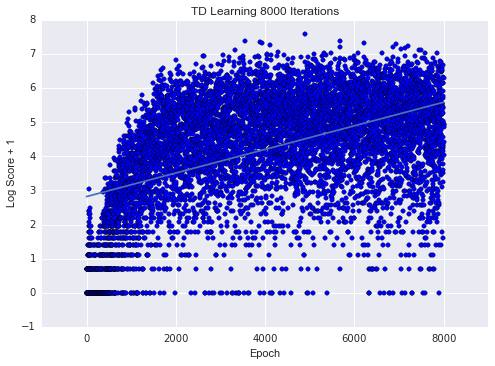
\includegraphics[scale=0.5]{td_8000_log}
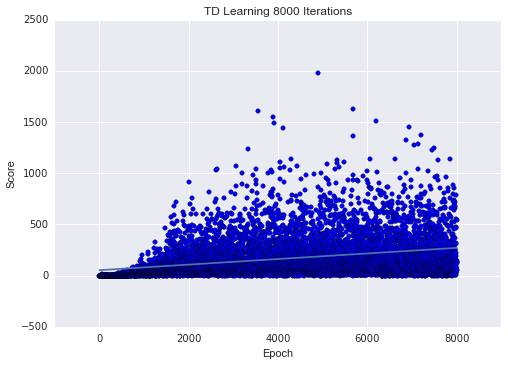
\includegraphics[scale=0.5]{TD_8000_score}
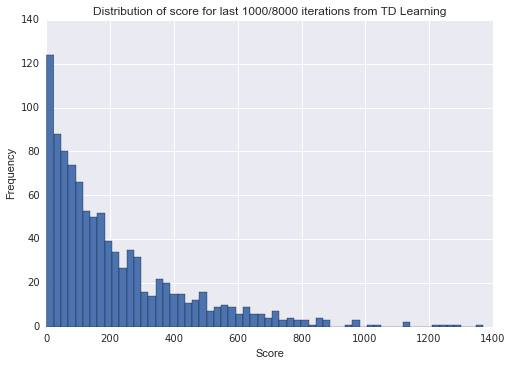
\includegraphics[scale=0.5]{td_8000_distribution}
\caption{Plot of score vs epoch for our TD-Learner, along with distribution of scores. Parameters used: $\alpha = 0.186493, \gamma = 1.0, p_h = 236, p_w = 530,p_v = 816$}
\label{fig:tdscore}
\end{figure}

\begin{figure}
\centering
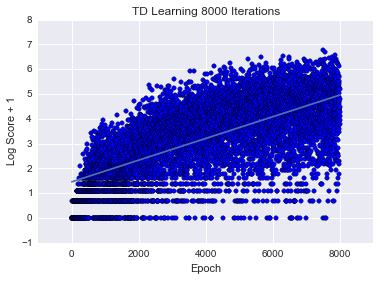
\includegraphics[scale=0.65]{TDQ_8000_log}
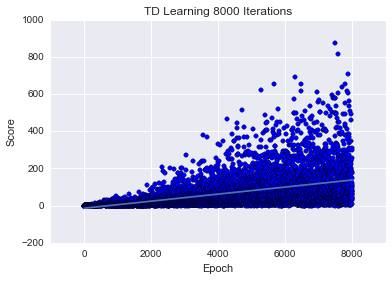
\includegraphics[scale=0.65]{TDQ_8000_score}
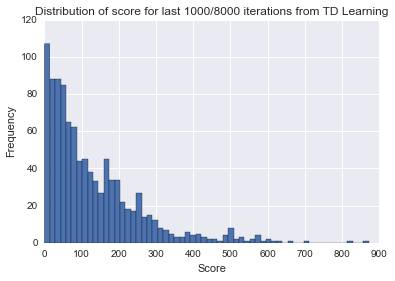
\includegraphics[scale=0.65]{TDQ_8000_distribution}
\caption{Plot of score vs epoch for our TD-Learner, along with distribution of scores. Parameters used: $\alpha = 0.15, \gamma = 0.95, p_h = 2, p_w = 2,p_v = 2$ (note these are the same as Figure \ref{fig:qscore})}
\label{fig:tdqscore}
\end{figure}

\begin{figure}
\centering
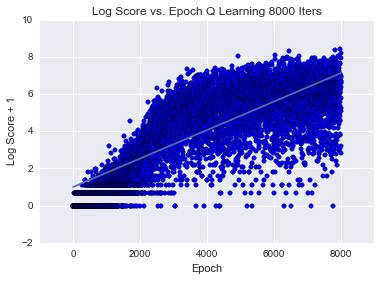
\includegraphics[scale=0.65]{Q_8000_log}
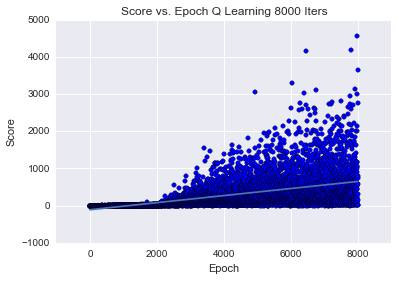
\includegraphics[scale=0.65]{Q_8000_score}
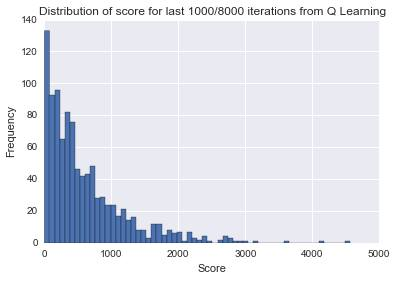
\includegraphics[scale=0.65]{Q_8000_distribution}
\caption{Plot of score vs epoch for our Q-Learner, along with distribution of scores. Parameters used: $\alpha = 0.15, \gamma = 0.95, p_h = 2, p_w = 2,p_v = 2$}
\label{fig:qscore}
\end{figure}

\subsection{Short-Term Learning}
We now turn our attention to the rate of learning. As discussed previously, we actually utilized the Spearmint software to obtain parameters over the first 200 iterations. The results are shown below in Figures \ref{fig:tdscore_small} (For TD-Learning) and \ref{fig:qscore_small} (For Q-Learning). It's incredible to see how quickly the monkey learns, in both models. For average statistics, we have that the Bayes optimized TD-Learner achieved a mean of 118.67 and median of 65.5 and the Bayes optimized Q-Learner achieved a mean of 44.5 and median of 26.5. \\

In this scenario, it's surprising to see that the Q-Learner is outperformed by the TD-Learner. We propose two possibilities for this:
\begin{itemize}
\item Propagation of negative reward. The TD-Learning algorithm will learn more quickly not to die. We can see that TD-Learning takes rises much more sharply at the beginning. However, this does not explain everything, since the score is actually an average of the final 100 epochs.
\item TD-Learner was optimized for a longer period of time using Spearmint. The optimization took over 300 data points, while the optimization for Q-Learner only utilized 156 data points. 
\end{itemize}
We lean towards the second explanation, given the fact that Q-Learner does much better than TD-Learner in the long-run for the purposes of our tests. 


\begin{figure}
\centering
\includegraphics[scale=0.5]{results_TDLearnerBayes_0}
\includegraphics[scale=0.5]{results_TDLearnerBayes_1}
\includegraphics[scale=0.5]{results_TDLearnerBayes_2}
\caption{Plot of Score vs Epoch for our TD-Learner with Bayes Optimization over 200 Epochs, along with distribution of scores. Parameters used: $\alpha = 0.303168, \gamma = 0.954306, p_h = 227.0, p_w = 442,p_v = 440$}
\label{fig:tdscore_small}
\end{figure}


\begin{figure}
\centering
\includegraphics[scale=0.5]{results_QLearnerBayes_0}
\includegraphics[scale=0.5]{results_QLearnerBayes_1}
\includegraphics[scale=0.5]{results_QLearnerBayes_2}
\caption{Plot of score vs epoch for our Q-Learner, along with distribution of scores. Parameters used: $\alpha = 0.368372, \gamma = 1.0, p_h = 16, p_w = 85,p_v = 1000$}
\label{fig:qscore_small}
\end{figure}




\section{Conclusion}
\label{sec:conclusion}
In conclusion, our analysis demonstrates a remarkable improvement of any method through the use of Bayesian parameter optimization. Given more computational resources and time, we are led to believe that optimizing the parameters for longer training periods (such as periods of 2048, 4096) and averaging over longer testing periods (such as 1024) would have led. For futher work, we would expect that allowing for more complex decay functions in the learning rate would improve the final results. In our preliminary tests with \textbf{qlearner4.py}, we already see some of these results. However, another area of interests would be to apply Dyna-Q or other non-converging algorithms to this problem. More research remains to be done into this particular problem, but from our results above, it seems that $\epsilon$-greedy $Q$-learning with optimized parameters using Spearmint perform well, learning both quickly and well in the long-run.\\

In conclusion, a Bayesian optimized Q-Learning algorithm appears to do well enough for the purposes of training the monkey to swing. 

% Reference section
\printbibliography

\end{document}